\documentclass[draft]{agujournal2019}
\usepackage{url}
\usepackage{lineno}
\usepackage[inline]{trackchanges} %for better track changes. finalnew option will compile document with changes incorporated.
\usepackage{soul}
\graphicspath{ {./fig/} }
\linenumbers

% \draftfalse

\journalname{Water Resources Research}


\begin{document}

\title{Evaluation of atmospheric model parameterization schemes with river network routing and streamflow observations: A case study of the Yarlung Zangbo River on the Tibetan Plateau}


\authors{Heng Yang\affil{1}, Shuanglong Chen\affil{2}, Qingyun Bian\affil{3}, and Hui Zheng\affil{4}}

\affiliation{1}{Science and Technology Research Institute, China Three Gorges Corporation, Beijing 100038, China}
\affiliation{2}{Baihetan Hydropower Plant, China Three Gorges Corporation, Sichuan 615421, China}
\affiliation{3}{IEIT Systems Co., Ltd., Beijing 100095, China}
\affiliation{4}{Institute of Atmospheric Physics, Chinese Academy of Sciences, Beijing 100029, China}

\correspondingauthor{Hui Zheng}{\url{hzheng_iap@outlook.com}}

\begin{keypoints}
      \item A river network routing-based method is developed to evaluate atmospheric models using streamflow observations
      \item High skill in streamflow correlation coefficient corresponds to superiority in modeling the spatial distribution of precipitation
      \item Shortwave radiation parameterization has a minimal impact on precipitation estimation but a notable impact on runoff and streamflow
\end{keypoints}


\begin{abstract}
      Evaluating kilometer-scale atmospheric models in data-sparse regions with complex topography, such as the Tibetan Plateau, presents inherent challenges due to the scarcity of in-situ observations and uncertainties in remote-sensing data. Hydrological evaluation, which utilize hydrological models to connect atmospheric model-simulated precipitation with streamflow observations, are hindered by model structural and parameter uncertainties, particularly significant in high-altitude mountainous basins. This study introduces a river network routing-based method that calculates streamflow directly from atmospheric model-simulated runoff, making fewer assumptions and thus being more adaptable to high-altitude mountainous basins. We applied this method to assess 3-kilometer Weather Research and Forecasting model simulations over the Yarlung Zangbo River on the Tibetan Plateau, each configured with distinct parameterizations for microphysics, planetary boundary layer, and shortwave radiation. The streamflow evaluation was compared with an evaluation of precipitation against satellite data. Results indicate that the streamflow evaluation complements the precipitation evaluation effectively. The WRF simulation that excelled in reproducing precipitation amounts and temporal variations also demonstrated the best performance in estimating streamflow's mean and variability. Furthermore, the river routing-based evaluation of streamflow offers additional insights beyond the precipitation evaluation. While the shortwave radiation parameterization had negligible impacts on precipitation amount, its influence on streamflow was significant. The experiment utilizing the Dudhia radiation scheme achieved the best temporal correlation with streamflow observations, corresponding to an accurate representation of spatial precipitation patterns as evaluated against satellite data. The findings underscore the value of the river network routing-based method in evaluating atmospheric models, especially in data-sparse and topographically complex regions.
\end{abstract}

\section{Introduction}
\label{sec:intro}

In recent years, the resolution of atmospheric models has gradually increased, reaching grid spacings as fine as 5 kilometers or less. These high-resolution, kilometer-scale models have largely overcome the need for deep convection parameterizations, thereby eliminating a significant source of uncertainty that was previously inherent in coarser-resolution models~\cite{prein2015RG, mooney2017JC}. Moreover, kilometer-scale atmospheric simulations are capable of capturing the intricate effects of fine-scale topography on atmospheric circulation patterns, particularly in mountainous regions~\cite{lin2018CD, zhou2021CD, yuan2023AR, sugimoto2021JHM, ma2023CD, li2022AAS}. The explicit representation of deep convection and meticulous attention to topographic detail have substantially enhanced the accuracy of the estimation of hydrological gradient along terrain slopes~\cite{jiang2022HESS, sugimoto2021JHM, ma2023CD}.

In mountainous regions characterized by strong hydrological gradients, such as the Tibetan Plateau, kilometer-scale atmospheric models are particularly useful~\cite{prein2023CD}. Mountainous regions experience pronounced hydrological gradients~\cite{immerzeel2014WRR} that are undergoing substantial changes due to global climate change~\cite{yao2019BAMS, cui2023NC, wang2021NCC, kraaijenbrink2021NCC}. The scarcity of in-situ observations and the inherent uncertainties in remote-sensing products impede the accurate monitoring of these hydrological changes~\cite{miao2024PNAS}. Evidence suggests that kilometer-scale atmospheric models can achieve an accuracy that surpasses that of in-situ observations \cite{lundquist2019BAMS} and even satellite-based products \cite{jiang2022IJC}. Moreover, these models are indispensable for projecting future water resources in the context of a changing climate \cite{prein2023CD}.

In mountainous regions, accurately evaluating kilometer-scale atmospheric models presents a formidable challenge. Meteorological observations are frequently confined to select locations within river valleys, leaving vast areas unmonitored. Remote locales, such as mountain peaks and barren lands, are known to contribute significantly to water sources but are often overlooked in observational data \cite{miao2024PNAS}. The complex topography and frozen ground in these areas can significantly distort remote-sensing products, including satellite-based precipitation estimates \cite{behrangi2014JAMC}. Consequently, the scarcity of in-situ meteorological observations and the associated uncertainties in remote-sensing data render the assessment of kilometer-scale atmospheric models less conclusive.

The concept of "doing hydrology backward"~\cite{kirchner2009WRR} has offered an enlightening method for evaluating atmospheric models in mountainous regions. This method involves using the precipitation simulated by an atmospheric model to drive a hydrological model, and then comparing the resulting streamflow with observed streamflow~\cite{krier2012WRR, henn2015WRR, henn2016WRR, pang2020HESS}. However, employing a hydrological model necessitates a substantial set of assumptions regarding model structure and parameters~\cite{kirchner2009WRR, henn2016WRR}. These assumptions can be tested in data-rich regions~\cite{clark2011WRR, zheng2020JAMES} but may falter in data-sparse regions, such as the Tibetan Plateau. To encompass the model's structural and parameter uncertainties, a diverse ensemble of model runs is essential to capture the spectrum of possible outcomes~\cite{henn2015WRR, vrugt2008WRR}. Yet, there exists the possibility that such uncertainties could be so pronounced that deriving precipitation from streamflow becomes an ill-posed problem~\cite{renard2010WRR}. This concern is particularly pertinent to high-altitude mountainous basins, such as the Yarlung Zangbo River basin, where considerable model structural and parameter uncertainty has been found in our previous study~\cite{lei2024JH}.

Despite the intricate nature of runoff-generation processes in mountainous regions~\cite{van_tiel2024NW}, the dynamics of water flow are often less complex than those observed over flat terrains~\cite{getirana2013WRR, moussa1996JH}. Characterized by steep slopes, mountain rivers enable water flow to be primarily represented using the kinematic wave approximation of the Saint-Venant equations~\cite{moussa1996JH}. This representation indicates that the flow is predominantly influenced by the interplay between friction and channel slope~\cite{getirana2013WRR, moussa1996JH}. Given that river channel slopes can be extracted globally from high-resolution digital elevation models~\cite{yamazaki2017GRL, yamazaki2019WRR}, the routing of water flow in mountainous basins is heavily reliant on assumptions about channel friction. While the friction assumption makes a relatively minor component within the previously discussed hydrological models,  characterizing uncertainties in channel friction is often more straightforward than addressing the structural and parameter uncertainties inherent to hydrological models. The simplicity and robustness of the routing process in mountainous basins enhance its adaptability for evaluating atmospheric models in these regions.

In the light of the aforementioned findings, we propose an alternative approach to evaluating atmospheric models that leverages river network routing. This approach involves directly routing the runoff simulated by atmospheric models through the river network to generate streamflow estimates at gauge locations. The method streamlines the evaluation process by circumventing the complexities of runoff generation processes, which are now integrated within the atmospheric model. The atmospheric models are capable of more effectively constraining the runoff generation processes than hydrological models, due to their ability to account for surface energy and water balance dynamics as well as land-atmosphere interactions~\cite{wagner2016WRR, senatore2015JAMES}. We contend that this river network routing-based method is particularly well-suited for data-sparse and topographically complex regions such as the Tibetan Plateau, providing a more targeted and effective means of model evaluation.

In this study, we have implemented our proposed method to evaluate the simulations produced by the Weather Research and Forecasting (WRF) model~\cite{powers2017BAMS}, specifically applied to the Yarlung Zangbo River, the most significant river on the Tibetan Plateau. The structure of this paper is as follows: Section~\ref{sec:methods} delineates the methodologies and datasets utilized within our research. Section~\ref{sec:results} details the outcomes and ensuing discussions. Finally, Section~\ref{sec:conclusions} synthesizes the findings and concludes the study.

\section{Methods and Data}
\label{sec:methods}

\subsection{Experimental Design}
\label{sec:design}

Figure~\ref{fig:workflow} illustrates the workflow of this study. We conducted a series of five 3-kilometer WRF experiments from May 1 to October 1, 2013, encompassing the wet season of the year. The experiments were configured with various parameterization schemes for cloud physics, planetary boundary layer, and shortwave radiation. The objective was to identify the optimal parameterization scheme using the streamflow observations from four river gauges along the Yarlung Zangbo River, namely Lazi, Nugesha, Yangcun, and Nuxia, arranged from upstream to downstream.

he WRF experiments were initialized and driven by data from the European Centre for Medium-Range Weather Forecasts Reanalysis version 5 (ERA5)~\cite{hersbach2020QJRMS}. Following this, the runoff simulated by WRF was spatially re-mapped to account for lateral inflow into the river network. The river flow within this network was then routed using the Muskingum method, a well-established approach for routing mountainous river flows. We tested a range of routing parameter values, calibrating them against streamflow observations to identify the optimal value for each segment of the river network situated between two river gauges. Subsequently, the WRF experiments were intercompared and assessed based on the accuracy of streamflow estimation using these optimal routing parameters.

\subsection{Observational Data}
\label{sec:data}

We utilized streamflow data provided by the China Three Gorges Corporation, collected at four river gauges along the Yarlung Zangbo River: Lazi, Nugesha, Yangcun, and Nuxia. Instantaneous streamflow observations were recorded at 00:00 UTC daily from June 20 to October 1, 2013. These data were instrumental in optimizing the routing parameter and evaluating the estimated streamflow for the WRF experiments.

To intercompare the river network routing-based evaluation of streamflow with the widely adopted precipitation evaluations based on remote sensing products, we also employed the Global Precipitation Measurement (GPM) Multi-satellitE Retrievals for GPM (IMERG) product~\cite{huffman2019GPM}. The IMERG product offers data at a spatial resolution of 0.1° by 0.1° and a temporal resolution of 30 minutes. We applied bilinear interpolation to downscale the GPM data to align with the 3-kilometer resolution of the WRF grid.

\begin{figure*}[h!]
      \centering
      \noindent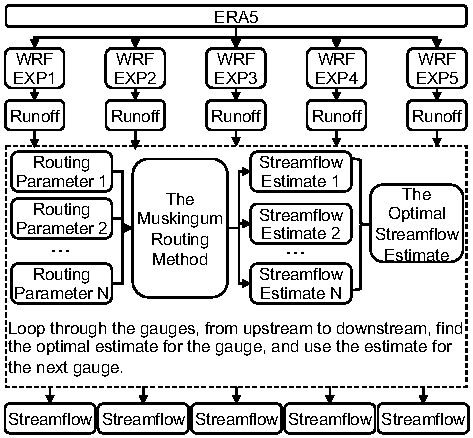
\includegraphics[width=140mm]{workflow.pdf}
      \caption{Schematic diagram of the workflow of this study.}
      \label{fig:workflow}
\end{figure*}

\subsection{Study Area and River Network}
\label{sec:domain}

Figure~\ref{fig:domain} displays the modeling domain of the WRF model, which spans 380 by 660 grid cells, each measuring 3 by 3 kilometers. The domain covers the entire Yarlung Zangbo River basin and extends to include a buffer zone that surrounds the river basin. This buffer zone, which is over 200 kilometers wide, is strategically designed to accommodate the development of small-scale weather systems before they interact with the river basin~\cite{denis2002CD}. This design helps to reduce the adverse effects stemming from inaccurate or low-resolution boundary conditions.

The routing was performed on the river network as illustrated in Figure~\ref{fig:domain}. The river network was delineated from the Multi-Error Removed Improved-Terrain Hydrography (MERIT-Hydro) dataset~\cite{yamazaki2017GRL, yamazaki2019WRR}, which offers flow directions and accumulative upstream area data at a spatial resolution of 3 by 3 arcseconds. The delineation process unfolds in three sequential steps: Initially, the accumulative upstream area is employed to identify river centerlines, with a grid cell being classified as such if its accumulative upstream area surpasses 10 km\textsuperscript{2}. Subsequently, these centerlines are segmented into river reaches from upstream to downstream, defining a reach by an increase in the ccumulative upstream area of at least 20 km\textsuperscript{2} along its path. Finally, the flow direction data is utilized to determine the catchment area of each reach, encompassing all grid cells that contribute flow directly to the reach. The thresholds for defining river centerlines and segmenting river reaches align with those used in previous large-domain river routing studies~\cite{lin2021SD, lin2019WRR}. This delineation process results in a fully connected river network consisting of 5,800 reaches.

\begin{figure*}[h!]
      \centering
      \noindent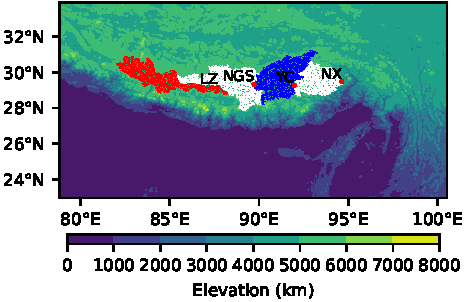
\includegraphics[width=140mm]{domain.pdf}
      \caption{Modeling Domain and Delineated River Network of the Yarlung Zangbo River. The colormap provides a representation of the terrain elevation, showcasing the basin's topographical characteristics. Red dots indicate the locations of the four river gauges along the river's course, labeled as follows: LZ for Lazi, NGS for Nugesha, YC for Yangcun, and NX for Nuxia from upstream to downstream. The differently colored lines correspond to the river reaches that lie between consecutive gauges, offering a visual guide to their spatial distribution across the basin.}
      \label{fig:domain}
\end{figure*}

\subsection{WRF Parameterization Schemes}
\label{sec:wrf}

Table~\ref{tab:wrf_experiment} lists the parameterization schemes chosen from WRF version 4.3.1 for the experiments. EXP1 serves as the baseline experiment, configured similarly to the High Asian Refined Analysis version 2~\cite{wang2021IJC} with the exception of the radiation and land surface processes. Instead of the Rapid Radiative Transfer Model (RRTM) scheme~\cite{mlawer1997JGRA}, the RRTM for GCMs (RRTMG)~\cite{iacono2008JGRA} was employed for shortwave and longwave radiation transfer. RRTMG is comparable to RRTM in terms of modeling radiative forcing but offers greater computational efficiency~\cite{iacono2008JGRA}. For the land surface processes, the Noah land surface model with multiparameterization options (Noah-MP)~\cite{niu2011JGRA,yang2011JGRA} was selected in place of the Noah model used in HARR version 2. Noah-MP has been enhanced over the original Noah model, providing an improved representation of snow and runoff processes~\cite{niu2011JGRA}. These enhancements have led to better performance in modeling runoff~\cite{liang2019AAS, zheng2023ESSD}, leading to the widespread adoption of Noah-MP in hydrological applications~\cite{cosgrove2024JAWRA, lin2018JHM}.

Building on EXP1, EXP2 through EXP5 are designed to investigate the impacts of cloud microphysics, planetary boundary layer, and shortwave radiation, one parameterization at a time. These parameterizations have demonstrated their significance in previous studies~\cite{lv2020JGRA, prein2023CD}. EXP2 and EXP3 vary from EXP1 in their cloud microphysics schemes. EXP1 employs the Thompson scheme~\cite{thompson2008MWR}, whereas EXP2 utilizes the Purdue Lin scheme~\cite{chen2002JMSJ}, and EXP3 incorporates the WRF Single-Moment 6-Class Microphysics (WSM6) scheme~\cite{hong2006APJAS}. EXP4 diverges from EXP1 in its planetary boundary layer scheme. Instead of the Mellor-Yamada-Janji'c scheme~\cite{janjic1994MWR}, EXP4 adopts the Yonsei University scheme~\cite{hong2006MWR}. EXP5 differs from EXP1 in its radiation scheme, opting for the Dudhia scheme~\cite{dudhia1989JAS} for shortwave radiation transfer.

\begin{table}[h!]
      \doublerulesep 0.3pt
      % \tabcolsep 7.8mm
      % \setlength{\tabcolsep}{15pt}   %%%设置表格平均分配列间距
      \renewcommand{\arraystretch}{1}  %%%设置表格行高
      \caption{WRF experiments and the used parameterization schemes.}
      \label{tab:wrf_experiment}
      \vspace*{5mm}
      \begin{tabular*}{140mm}{cccc}
            \hline
            Experiment & Cloud Microphysics & Planetary Boundary Layer & Shortwave Radiation \\
            \hline
            EXP1 & Thompson & MYJ & RRTMG \\
            EXP2 & Purdue Lin & MYJ & RRTMG \\
            EXP3 & WSM6 & MYJ & RRTMG \\
            EXP4 & Thompson & YSU & RRTMG \\
            EXP5 & Thompson & YSU & Dudhia \\
            \hline
      \end{tabular*}
      \renewcommand{\arraystretch}{1}  %%%设置表格行高
\end{table}

\subsection{River Network Routing Method}
\label{sec:river}

The WRF-simulated runoff is re-mapped to represent lateral inflow into the rivers, ollowing the remapping method detailed in \cite{lin2018EMS, wang2019CSB}. For each river reach within the network, the WRF grid cells that intersect with the catchment area of the reach are first identified. The runoff volume from these grid cells is then calculated by multiplying the runoff depth by the area of intersection for each cell. These individual values are subsequently summed to ascertain the total lateral flow volume entering the reach. Given the steep topography and extensive watershed area characteristic of the study region, terrain routing is intentionally omitted in this study to focus on the primary river flow dynamics and streamline the computational process.

We employ the Muskingum method to route water flow within the river network. This method is well-suited to characterize the flow's kinematic wave propagation that driven by the topographic gradient~\cite{ponce1978JHD}. The formulation of the Muskingum method~\cite{cunge1969JHD, fenton2019JH}, when incorporating lateral inflows, can be expressed as follows:
\begin{eqnarray}
      Q_{i}^{t} = \frac{k - x}{1 - x + k} Q_{i-1}^{t} + \frac{1 - x - k}{1 - x + k} Q_{i}^{t-1} + \frac{x + k}{1 - x + k} Q_{i-1}^{t-1} + \frac{2k}{1 - x + k} Q_l^t \textrm{,} \label{eq:muskingum}\\
      k  = \frac{c \Delta t} {2 \Delta l} \textrm{,}
\end{eqnarray}
where $Q_{i}^{t}$ ($\textrm{m}^3\,\textrm{s}^{-1}$) is the streamflow of a reach at current time step, $Q_{i-1}^{t}$ ($\textrm{m}^3\,\textrm{s}^{-1}$) is the streamflow at the upstream position of the reach at current time step, $Q_{i}^{t-1}$ ($\textrm{m}^3\,\textrm{s}^{-1}$) is the streamflow of the reach at previous time step, $Q_{i-1}^{t-1}$ ($\textrm{m}^3\,\textrm{s}^{-1}$) is the streamflow at the upstream position at the previous time step, $Q_l^t$ ($\textrm{m}^3\,\textrm{s}^{-1}$) is the lateral inflow entering the reach at current time step. $\Delta t$ is the time step ($\textrm{s}$), and $\Delta l$ is the reach length ($\textrm{m}$). $x$ is the weighting factor (unitless), and $c$ is the wave celerity ($\textrm{m}\,\textrm{s}^{-1}$).

The application of the Muskingum method to the reaches of a fully connected river network must be executed in the correct order. When routing the streamflow of a reach, the discharge at the reach's upstream position must be available. We sorted all the river reaches with the network according to the stream order as introduced in \cite{yang2024W}. This sorting ensures that upstream reaches are always prioritized over their downstream reaches. Subsequently, we apply the Muskingum method to each reach in the established sequence. This sequence guarantees that routing on upstream reaches is conducted first, followed by routing on downstream reaches.

The Muskingum method includes two adjustable routing parameters: the weighting factor ($x$; unitless) and wave celerity ($c$; $\textrm{m},\textrm{s}^{-1}$). The weighting factor $x$ is used to regulate the proportional contributions of the right-hand-side terms in Equation~\ref{eq:muskingum}. Studies have shown that the simulated streamflow is relatively insensitive to variations in the weighting factor~\cite{koussis1978JHD}. Values ranging from 0.1 to 0.3 are typically effective for most streams. Guided by the experiments reported by \citeA{david2011JHM}, we have chosen a parameter value of 0.3 for this study."

The wave celerity $c$ represents the speed at which the flow wave propagates downstream and is influenced by the physical characteristics of the river channel, including channel slope, roughness, and width. Given that direct observations of $c$ are unavailable for the Yarlung Zangbo River basin, we conducted a series of simulations with varying wave celerity values. We selected the value that best aligns with the streamflow observations, which is considered representative of the river channel's physical characteristics. The optimal wave celerity value $c$ is determined for each streamflow gauge in an upstream-to-downstream sequence. Once a wave celerity value is chosen for a gauge, it is applied to all downstream gauges. This process is repeated sequentially until wave celerity values are selected for all streamflow gauges.

\subsection{Evaluation Metrics}
\label{sec:metrics}

We utilized the Pearson correlation coefficient to identify the optimal wave celerity value. The Pearson correlation coefficient ($r$) is defined as follows:
\begin{equation}
      r = \frac{\sum_{i=1}^{n} (x_i - \bar{x})(y_i - \bar{y})}{\sqrt{\sum_{i=1}^{n} (x_i - \bar{x})^2 \sum_{i=1}^{n} (y_i - \bar{y})^2}} \textrm{,}
\end{equation}
where $x_i$ and $y_i$ are the simulated and observed streamflow at time step $i$, respectively. $\bar{x}$ and $\bar{y}$ are the mean of the simulated and observed streamflow, respectively. The Pearson correlation coefficient ranges from \textminus{}1 to 1, with a value of 1 indicating a perfect positive linear relationship between the simulated and observed streamflow. This coefficient is insensitive to biases in the streamflow estimates, making us to focus on daily scale streamflow variations in this study.

We used the Kling--Gupta efficiency (KGE)~\cite{gupta2009JH} to intercompare the WRF parameterization schemes. KGE sythematically summarizes how a hydrological simulation matches observations in correlation, standard deviation, and bias. The KGE is defined as follows:
\begin{eqnarray}
      \textrm{KGE} = 1 - \sqrt{\left(r - 1\right)^2 + \left(\alpha  - 1\right)^2 + \left(\beta - 1\right)^2} \textrm{,} \\
      \alpha  = \frac{\sigma}{\sigma_o} \textrm{,}                                                                 \\
      \beta = \frac{\mu_s}{\mu_o} \textrm{,}
\end{eqnarray}
where $r$ is the Pearson correlation coefficient between the simulation and observation, $\sigma$ is the standard deviation of the simulation, and $\mu$ is the mean. The subscripts $s$ and $o$ denote the simulated and observed values, respectively. The KGE ranges from $-\infty$ to 1. A KGE value of 1 indicates a perfect match between the simulated and observed streamflow.

\section{Results and Discussion}
\label{sec:results}

In this section, we first intercompares the WRF-simulated precipitation and runoff. Subsequently, we assess the streamflow estimates by comparing them against observed streamflow data.

\subsection{Intercomparison of the WRF-simulated precipitation and runoff}

Figure~\ref{fig:prdist} displays the spatial distribution of simulated precipitation from the five WRF experiments. The patterns from EXP1 through EXP3 exhibit close agreement, with two primary precipitation centers evident downstream of Yangcun and between Lazi and Nugesha. Notably, the precipitation intensity between Lazi and Nugesha is slightly higher. In comparison to the baseline EXP1, the distribution in EXP5 appears more dispersed, featuring a significant precipitation center downstream of Yangcun, as shown in Figure~\ref{fig:prdist}e. EXP4 closely mirrors the spatial pattern of EXP5, with a spatial correlation coefficient of 0.93 achieved between them. However, EXP4 (Figure~\ref{fig:prdist}d)exhibits the weakest precipitation intensity among the experiments. The experiments show greater consensus in the downstream areas of the Yarlung Zangbo River than in the headwater regions, as indicated in Figure~\ref{fig:prdist}f. When juxtaposed with the GPM data, there is a tendency for all five experiments to overestimate the precipitation rate.

\begin{figure*}[h!]
      \centering
      \noindent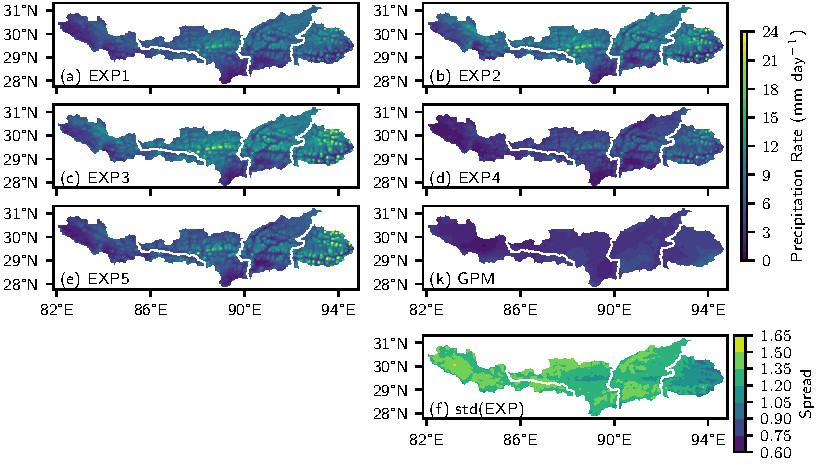
\includegraphics[width=140mm]{prrn_prdist.pdf}
      \caption{Spatial distribution of the precipitation rate averaged from June 20 to October 1, 2013. (a)--(e) The five WRF experiments described in Table~\ref{tab:wrf_experiment}. (k) The GPM precipitation. (f) the ensemble spread of the five experiments measured in standard deviation. The white lines denotes the division of the river network between two river gauges. \label{fig:prdist}}
\end{figure*}

Figure~\ref{fig:prcumupts} presents the time series of accumulated precipitation, averaged across the catchments of the four river gauges. Consistent with the spatial distribution depicted in Figure~\ref{fig:prdist}, all five WRF experiments exceed the GPM precipitation rate across all four catchments. The variation among the experiments is considerable. The disparity between EXP4 and EXP1 underscores the significant influence of the planetary boundary layer on precipitation. This finding aligns with the results reported by \citeA{prein2023CD}, suggesting that the impact of planetary boundary layer parameterization can be more pronounced than that of cloud physics, as evidenced by the differences between EXP1 and EXP2, and between EXP1 and EXP3. The difference between EXP5 and EXP1 is negligible across all four catchments, indicating that the parameterization of shortwave radiation has a minimal impact on the simulation of precipitation.

\begin{figure*}[h!]
      \centering
      \noindent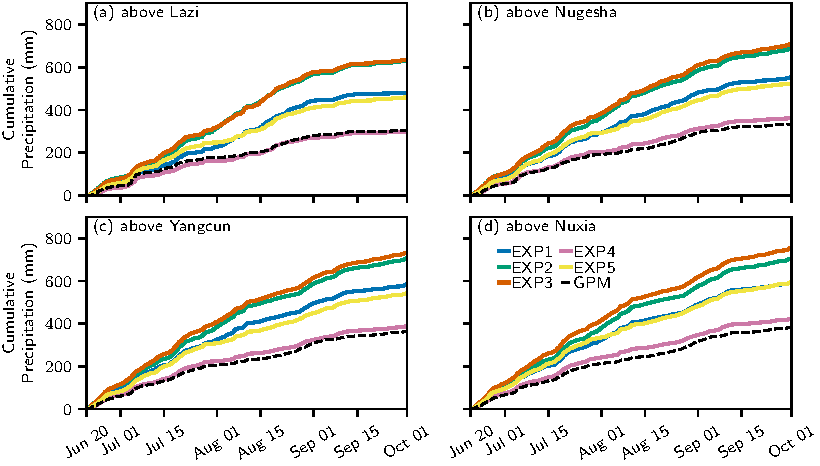
\includegraphics[width=140mm]{prrn_prcumupts.pdf}
      \caption{Time series in the accmulated precipitation averaged over the areas above (a) Lazi, (b) Nugesha, (c) Yangcun, and (d) Nuxia. \label{fig:prcumupts}}
\end{figure*}

Table~\ref{tab:pr_skill} presents the skill of the WRF experiments as measured against GPM data. The cloud physics parameterization significantly influences the timing of precipitation, leading to substantial changes in the correlation coefficient ($r$) for EXP2 and EXP3 relative to EXP1. A comparison between EXP4 and EXP1 indicates that the planetary boundary layer parameterization has a minimal impact on precipitation timing. However, there are notable differences in the amount of precipitation ($\beta$) and its variability ($\alpha$), suggesting the importance of the planetary boundary layer in moisture transport for precipitation~\cite{wang2020GRL}. Although the shortwave radiation parameterization has a minimal impact on the amount of precipitation ($\beta$), it significantly affects the magnitude of precipitation variability ($\alpha$), particularly in the middle reaches of the Yarlung Zangbo River between Lazi and Yangcun. The reason for this impact is not yet clear. However, offline studies in this area~\cite{lei2024JH} have found that shortwave radiation significantly affects the land surface energy and water budgets. We hypothesize that the changes in precipitation may be a consequence of local land-atmosphere interactions originated from the changes in land surface energy budgets.

\begin{table}[h!]
      \centering
      \doublerulesep 0.3pt
      % \tabcolsep 7.8mm
      % \setlength{\tabcolsep}{15pt}   %%%设置表格平均分配列间距
      \renewcommand{\arraystretch}{1}  %%%设置表格行高
      \caption{Kling--Gupta efficiency of the hourly precipitation rate averaged within the catchment of the river gauges. Italic fonts indicate the experiment that best matches GPM.}
      \label{tab:pr_skill}
      \vspace*{5mm}
      \small
      \begin{tabular*}{80mm}{cccccc}
            \hline
            & Metric & LZ & NGS & YC & NX \\
            \hline
            EXP1 & KGE & 0.32 & 0.25 & 0.30 & 0.36 \\
            & $\alpha$ & 1.06 & 1.22 & 1.22 & 1.22 \\
            & $\beta$ & 1.58 & 1.66 & 1.60 & 1.55 \\
            & $r$ & 0.65 & 0.72 & 0.73 & 0.75 \\
            \\
            EXP2 & KGE & \textminus{}0.23 & \textminus{}0.22 & \textminus{}0.10 & 0.00 \\
            & $\alpha$ & 1.27 & 1.39 & 1.37 & 1.37 \\
            & $\beta$ & 2.07 & 2.06 & 1.94 & 1.85 \\
            & $r$ & 0.46 & 0.53 & 0.56 & 0.60 \\
            \\
            EXP3 & KGE & \textminus{}0.19 & \textminus{}0.23 & \textminus{}0.12 & \textminus{}0.07 \\
            & $\alpha$ & 1.22 & 1.36 & 1.34 & 1.34 \\
            & $\beta$ & 2.08 & 2.12 & 2.01 & 1.97 \\
            & $r$ & 0.58 & 0.65 & 0.67 & 0.69 \\
            \\
            EXP4 & KGE & \textit{0.61} & \textit{0.72} & \textit{0.73} & \textit{0.75} \\
            & $\alpha$ & 0.75 & \textit{0.94} & \textit{0.94} & \textit{0.97} \\
            & $\beta$ & \textit{0.98} & \textit{1.09} & \textit{1.07} & \textit{1.11} \\
            & $r$ & \textit{0.70} & \textit{0.74} & \textit{0.75} & \textit{0.77} \\
            \\
            EXP5 & KGE & 0.39 & 0.35 & 0.42 & 0.38 \\
            & $\alpha$ & \textit{0.94} & 1.11 & 1.09 & 1.14 \\
            & $\beta$ & 1.51 & 1.57 & 1.49 & 1.55 \\
            & $r$ & 0.67 & 0.72 & 0.71 & 0.74 \\
            \hline
      \end{tabular*}
      \renewcommand{\arraystretch}{1}  %%%设置表格行高
\end{table}

Figure~\ref{fig:rncumupts} presents the time series of accumulated runoff, averaged across the catchments of the four river gauges. The accumulated runoff for the specified period correlates well with the precipitation data. The accumulated runoff for the specified period exhibits a strong correlation with the precipitation data. Among the five experiments, EXP2 and EXP3 produce the highest runoff estimates, with their performances being closely aligned. In contrast, EXP4 records the lowest runoff, and its deviation from EXP1 is more significant than the difference observed between EXP1 and EXP2. The disparity in runoff between EXP5 and EXP1 is considerably larger than the difference in their respective precipitation estimates, especially in the upper reaches of the Yarlung Zangbo River, as shown in Figures~\ref{fig:rncumupts}b and \ref{fig:rncumupts}c. This pronounced difference in runoff is anticipated to result in variations in the streamflow estimates, which will be further analyzed in the subsequent sections.

\begin{figure*}[h!]
      \centering
      \noindent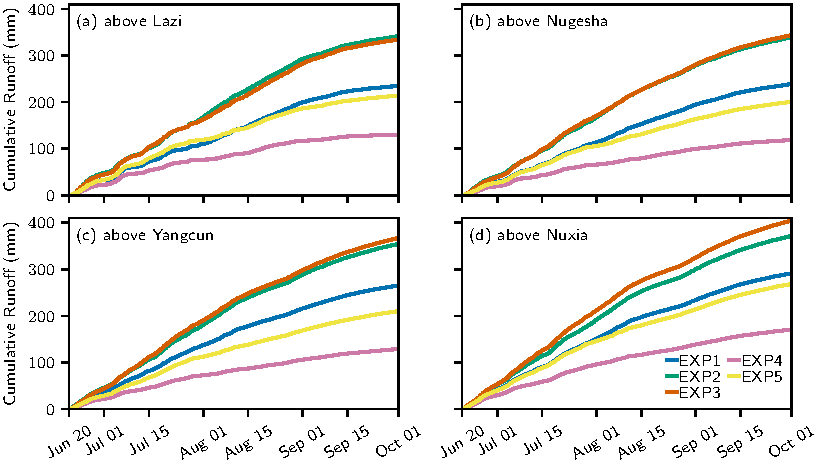
\includegraphics[width=140mm]{prrn_rncumupts.pdf}
      \caption{Time series in the accmulated runoff averaged over the areas above (a) Lazi, (b) Nugesha, (c) Yangcun, and (d) Nuxia. \label{fig:rncumupts}}
\end{figure*}

\subsection{Evaluation against streamflow observations}

Figure~\ref{fig:celerity} demonstrates the changes in the correlation coefficient of streamflow with celerity across the four river gauges. Table~\ref{tab:celerity} lists the optimal celerity values for each gauge corresponding to the WRF experiments. The variation of the correlation coefficient with celerity and the optimal celerity values exhibit consistency across all five experiments. This consistency supports the notion that celerity is predominantly determined by the river channel characteristics in mountainous basins. Specifically, the optimal celerity in the upstream segment of the main channel is generally slower compared to that in the downstream segment. As shown in Figure~\ref{fig:domain}, the downstream area, located at the edge of the Tibetan Plateau, is characterized by a broader river channel and a more pronounced slope, which likely contributes to the observed celerity differences.

\begin{figure*}[h!]
      \centering
      \noindent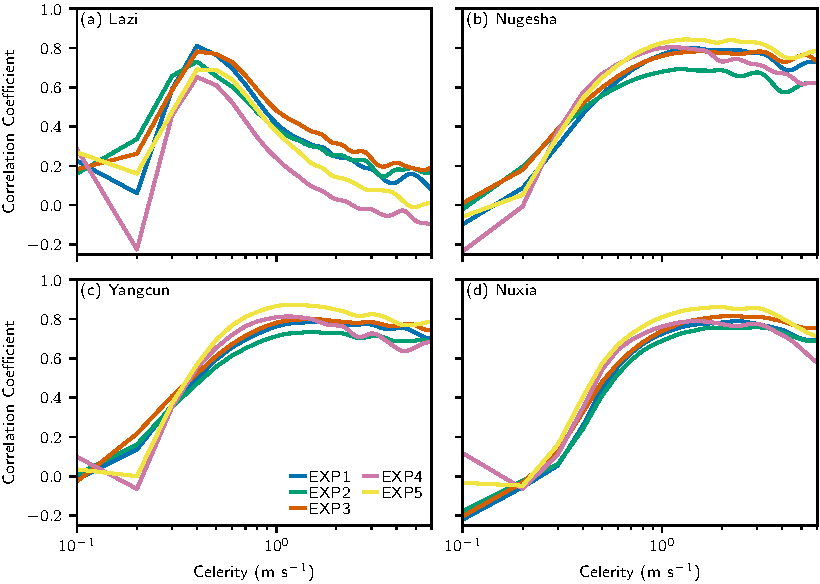
\includegraphics[width=140mm]{q_sens_cc.pdf}
      \caption{Sensitivity of streamflow modeling skill to wave celerity at the four river gauges. (a) Lazi, (b) Nugehsa, (c) Yangcun, and (d) Nuxia. \label{fig:celerity}}
\end{figure*}

\begin{table}[h!]
      \centering
      \doublerulesep 0.3pt
      % \tabcolsep 7.8mm
      % \setlength{\tabcolsep}{15pt}   %%%设置表格平均分配列间距
      \renewcommand{\arraystretch}{1}  %%%设置表格行高
      \caption{The optimal flow wave celerity.}
      \label{tab:celerity}
      \vspace*{5mm}
      \small
      \begin{tabular*}{50mm}{ccccc}
            \hline
            & LZ & NGS & YC & NX \\
            \hline
            EXP1 & 0.4 & 1.4 & 1.5 & 2.4 \\
            EXP2 & 0.4 & 1.2 & 1.5 & 3.0 \\
            EXP3 & 0.4 & 1.6 & 1.5 & 2.2 \\
            EXP4 & 0.4 & 1.1 & 1.2 & 1.5 \\
            EXP5 & 0.4 & 1.3 & 1.2 & 1.9 \\
            \hline
      \end{tabular*}
      \renewcommand{\arraystretch}{1}  %%%设置表格行高
\end{table}

Figure~\ref{fig:q_opt} displays the time series of streamflow estimates for the five WRF experiments at the four river gauges. Table~\ref{tab:rn_skill} provides a detailed assessment of the skill of these estimations. Consistent with the observations in precipitation and runoff, there are notable differences in streamflow estimates among the experiments. While EXP4 demonstrated the best performance across all metrics in the evaluation of precipitation against GPM, its advantage in streamflow is primarily observed in terms of bias and in the Kling-Gupta Efficiency (KGE) at the upper to middle reaches. The KGE value for EXP4 increases progressively from upstream to downstream, with a value of -1.78 at the Lazi gauge and improving to 0.69 at the Yangcun gauge. At the most downstream gauge, Nuxia, EXP5 outperforms EXP4, achieving a KGE value of 0.70.

It is noteworthy that EXP5 outperforms EXP1 except at the upstream position of the Yarlung Zangbo River at Lazi, even though their precipitation amounts are quite similar. This superior performance of EXP5 is primarily attributed to the improved correlation coefficient between the simulated and observed streamflow time series. We have examined the relationship between the spatial correlation coefficient of streamflow and the catchment-wide spatial correlation coefficient of precipitation, as depicted in Figure~\ref{fig:q_cc_p}. With the exception of the Lazi catchment, a relatively high correspondence in the temporal variations of streamflow is well-aligned with a relatively high correspondence in the spatial distribution of precipitation. This alignment is a consequence of water flow from various locations within the catchment converging at the catchment outlet, which influences the overall streamflow dynamics.

\begin{figure*}[h!]
      \centering
      \noindent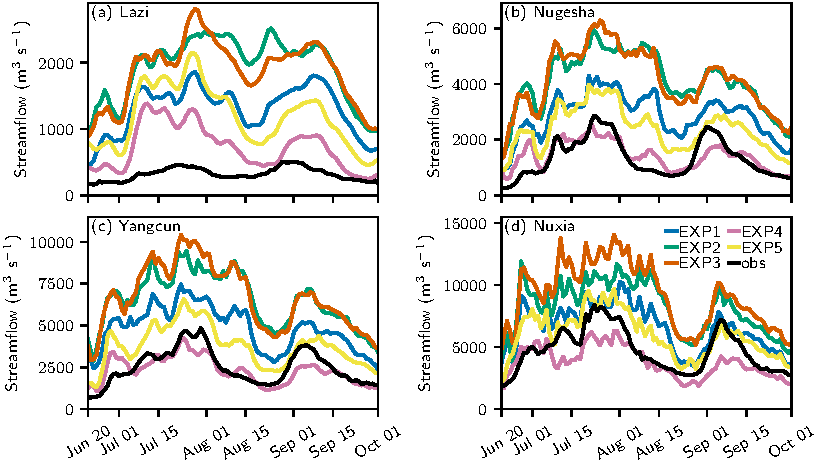
\includegraphics[width=140mm]{q_opt.pdf}
      \caption{Comparison between streamflow observations and the streaflow estimated from the WRF experiments. \label{fig:q_opt}}
\end{figure*}

\begin{table}[h!]
      \centering
      \doublerulesep 0.3pt
      % \tabcolsep 7.8mm
      % \setlength{\tabcolsep}{15pt}   %%%设置表格平均分配列间距
      \renewcommand{\arraystretch}{1}  %%%设置表格行高
      \caption{Kling--Gupta efficiency of the optimal streamflow estimate.}
      \label{tab:rn_skill}
      \vspace*{5mm}
      \small
      \begin{tabular*}{80mm}{cccccc}
            \hline
            & Metric & LZ & NGS & YC & NX \\
            \hline
            EXP1 & KGE & \textminus{}3.12 & \textminus{}0.16 & 0.01 & 0.54 \\
            & $\alpha$ & 3.76 & 1.14 & 1.26 & 1.06 \\
            & $\beta$ & 4.05 & 2.14 & 1.93 & 1.40 \\
            & $r$ & \textit{0.81} & 0.80 & 0.79 & 0.79 \\
            \\
            EXP2 & KGE & \textminus{}5.34 & \textminus{}1.16 & \textminus{}0.72 & 0.19 \\
            & $\alpha$ & 4.88 & 1.51 & 1.57 & 1.23 \\
            & $\beta$ & 6.00 & 3.08 & 2.60 & 1.74 \\
            & $r$ & 0.73 & 0.69 & 0.74 & 0.76 \\
            \\
            EXP3 & KGE & \textminus{}5.24 & \textminus{}1.21 & \textminus{}0.88 & \textminus{}0.09 \\
            & $\alpha$ & 4.95 & 1.65 & 1.84 & 1.51 \\
            & $\beta$ & 5.82 & 3.11 & 2.67 & 1.95 \\
            & $r$ & 0.78 & 0.78 & 0.80 & 0.82 \\
            \\
            EXP4 & KGE & \textit{\textminus{}1.78} & \textit{0.65} & \textit{0.69} & 0.60 \\
            & $\alpha$ & \textit{3.46} & 0.72 & 0.77 & 0.72 \\
            & $\beta$ & \textit{2.25} & \textit{1.07} & \textit{0.93} & \textit{0.81} \\
            & $r$ & 0.65 & 0.80 & 0.81 & 0.79 \\
            \\
            EXP5 & KGE & \textminus{}3.59 & 0.19 & 0.45 & \textit{0.70} \\
            & $\alpha$ & 4.71 & \textit{1.13} & \textit{1.17} & \textit{1.04} \\
            & $\beta$ & 3.68 & 1.79 & 1.51 & 1.27 \\
            & $r$ & 0.69 & \textit{0.84} & \textit{0.87} & \textit{0.86} \\
            \hline
      \end{tabular*}
      \renewcommand{\arraystretch}{1}  %%%设置表格行高
\end{table}


\begin{figure*}[h!]
      \centering
      \noindent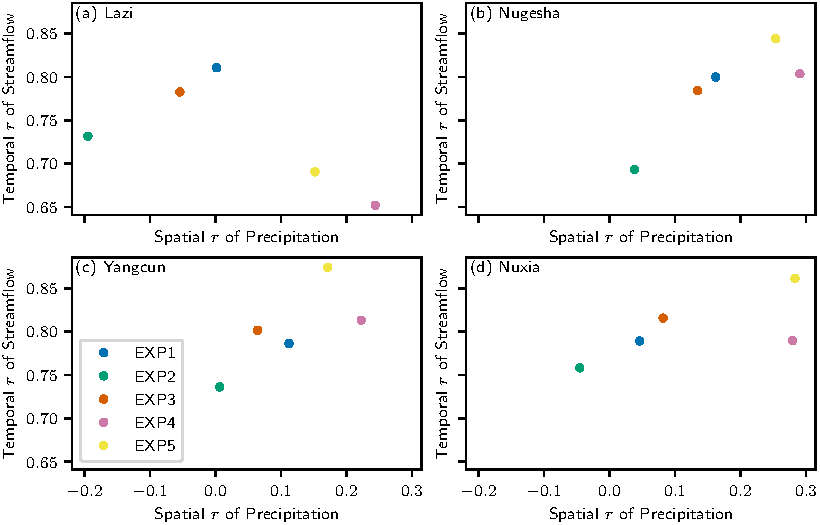
\includegraphics[width=140mm]{q_cc_p.pdf}
      \caption{Relationship between the spatial correlation coefficient of precipitation and temporal correlation coefficient of streamflow. (a) The streamflow observed at Lazi and the precipitation averaged in the catchment of Lazi, (b) for Nugesha, (c) for Yangcun, and (d) for Nuxia. \label{fig:q_cc_p}}
\end{figure*}

\section{Conclusions}
\label{sec:conclusions}

We have proposed a river network routing-based method for evaluating atmospheric models using streamflow observations. This method stands out from the hydrological model-based approach by relying on a substantially smaller set of assumptions regarding model structures and parameters. The streamlined nature of this approach bolsters its robustness and, in comparison to hydrological model-based evaluations, offers a more attractive alternative. This is especially true in mountainous basins, where the intricacies of runoff-generation processes frequently surpass the modeling capabilities of hydrological models.

We applied this method to evaluate five numerical experiments, each featuring different configurations of WRF, in the simulated streamflow of the Yarlung Zangbo River, the largest river on the Tibetan Plateau. The streamflow evaluation complements the precipitation evaluation utilizing the GPM precipitation product. Our results indicate a consistency between the proposed method's outcomes and those derived from the precipitation evaluation. Notably, the WRF configuration that integrated the Thompson cloud microphysics scheme, the RRTMG radiation scheme, and the YSU planetary boundary layer scheme exhibited optimal performance in simulating precipitation. This configuration's enhanced capability to replicate both the total amount and temporal patterns of precipitation is crucial for accurately estimating the mean and variability of streamflow.

Our proposed method enriches the evaluation of precipiattion. While the shortwave radiation transfer process was found to have a minimal impact on the total amount of precipitation during the initial evaluation, it exerts a significant influence on streamflow simulation, particularly in the middle reaches between Lazi and Yangcun. Notably, the experiment that employed the Dudhia radiation scheme excelled in terms of the correlation coefficient and the Kling-Gupta Efficiency (KGE) at the downstream Nuxia gauge. This superior performance in modeling streamflow time series is attributed to the Dudhia scheme's effectiveness in capturing the spatial distribution of precipitation, underscoring the importance of accurate radiation transfer modeling in streamflow simulation. These findings reinforce the significance of the precipitation gradient in mountainous hydrology, as discussed in \cite{immerzeel2014WRR}, and demonstrate the potential of our proposed method in evaluating atmospheric models in mountainous basins.

\section*{Open Research Section}

The GPM precipitation data were retrieved from \url{https://doi.org/10.5067/GPM/IMERG/3B-HH/06}. The ERA5 reanalysis data are obtained from the ECMWF climate data store, accessible via the following DOIs: \url{https://doi.org/10.24381/cds.bd0915c6} and \url{https://doi.org/10.24381/cds.adbb2d47}. The WRF model, version 4.3.1, is available at the model's official repository on GitHub: \url{https://github.com/wrf-model/WRF}. The MERIT-Hydro flow direction and cumulative upstream area data can be accessed at the following web address: \url{http://hydro.iis.u-tokyo.ac.jp/~yamadai/MERIT_Hydro/}. The delineated river network and WRF-simulated precipitation and runoff can be found on Science Data Bank (\url{https://doi.org/10.57760/sciencedb.11618}). The streamflow observations for the Yarlung Zangbo River were obtained from China Three Gorges Corporation; however, they are not shareable due to licensing restrictions. The routing code used in this study is available at the GitHub repository: \url{https://github.com/hzheng88/paper-2024-yaluzangbu-wrf-streamflow}.

\acknowledgments

This study is supported by China Three Gorges Corporation (contract Z532302035) and the Natural Science Foundation of China (grants 42075165 and 42275178).

\bibliography{references}

\end{document}
